%\documentclass[class=article, crop=false]{standalone}
\documentclass{article}

\title{Introduction}
\author{Anna Borri}
% \date{August 2025}

%%%%%%%%%%%%% LANGUAGE AND BIBLIOGRAPHY %%%%%%%%%%%%%%%%%
%%% Allows the use of accented characters
\usepackage[T1]{fontenc} %come sot\to

%%% Allows typing accented characters directly
\usepackage[utf8]{inputenc} %aggiunge caratteri accentati

\usepackage[main=english]{babel} %lingua

%%% Bubliography
\usepackage[style=alphabetic]{biblatex}
\addbibresource{bibliography.bib} %specifica il file della bibliografia

\renewcommand\mkbibnamefamily[1]{\textsc{#1}} %autori in maiuscoletto
\usepackage{csquotes}



%%%%%%%%%%%%%%%%%%%%%%%%%%%%%%%%%%%%%%%%%%%%%%%%%%%%%%%%%%%%%%%%%%%%%%%%%%%%%%%%%%%%%%%%%%%%%%%%%%%%%%%%%%%%%%%%%%%%%%%%%%%%%%%%%%%%%%%%%%%%%%%%%%%%%%%%%%%%%%%%%%%%%%%%%%%%%%%%%%%%%%%%%%%%%%%%%%%

%%%%%%%%%%% PLOTTING AND GRAPHICS %%%%%%%%%%%%%%%%
%%% Plot graphs
% \usepackage{pgfplots}
% \pgfplotsset{compat=1.15}

%%% Include images
\usepackage{graphicx}

\usepackage{tikz-cd}
\usetikzlibrary{arrows}

\usepackage{quiver}

\usepackage{tikz}
\usetikzlibrary{calc, arrows.meta, positioning, patterns}

%%%%%%%%%%% MATH AND SYMBOLS %%%%%%%%%%%%%%%%%%
%%% Math fonts and symbols
\usepackage{amsfonts,amssymb}

% %%% Needed for \mathbb, i.e. for the characteristic function symbol
% \usepackage[bb=dsserif]{mathalpha}

%%% Use \mathscr{}
\usepackage{mathrsfs}

%%% Special mathematical symbols
\usepackage{stmaryrd}

%%% Enhanced math environments, like align, gather...
\usepackage{amsmath}

%% Extension of amsmath with extra math symbols, alignment tools, and fixes. Automatically loads amsmath
\usepackage{mathtools}
\mathtoolsset{showonlyrefs,showmanualtags} %% Numbers only equations that are referenced. Allows manual tagging without being overridden by automatic numbering.
\numberwithin{equation}{section} %% Equations are numbered according to the section

%%% Put labels over symbols. Already part of amsmath
%\usepackage{stackrel}

%%% Theorem environments
\usepackage{amsthm}

%%% Relative font sizing in math (\mathlarger{...}), for example to make sums bigger
% \usepackage{relsize}

%%% Draw cancel lines through terms, for simplifying expression. Contains the command \cancel{}
% \usepackage{cancel}


%%%%%%%%%%%% LAYOUT AND FORMATTING %%%%%%%%%%%%%%%%%%%%%
%%% Fine control of figure/table placement ([H] option)
\usepackage{float}

%%% Resize, scale, trim boxes (including images and tables). Contains the command \adjustbox
\usepackage{adjustbox}

%%% Customizes lists (itemize, enumerate) spacing and labels.
\usepackage{enumitem}

%%% Verbatim (code/text) blocks without formatting.
\usepackage{verbatim}
% The verbatim environment prints text exactly as typed: every character (including \ { } % # _ ^ ~), spaces, and line breaks are preserved. The command is \begin{verbatim} \end{verbatim}.

%%% Comment big portions of text with \begin{comment} \end{comment}
\usepackage{comment}

%%%%%%%%%% MANAGING REFERENCES %%%%%%%%%%%%%%%%%%%%
\usepackage{zref-clever} % Allows to automatically add the type of the reference with the command \zcref{}. It is also compatible with equations
\zcsetup{capfirst} % Option of zref-clever to ca\pitalize the first letter of the referenced statement with \zcref{}

\usepackage{hyperref} % Classical references manager. Contains the \eqref{} command, which completes the referred equation with parentheses (e.g. (2)), but doesn't write the type like \zcref{} (e.g. Equation(2))
\hypersetup{
  colorlinks,
  citecolor=magenta,
  linkcolor=black,
  urlcolor=blue}%NB da caricare per ultimo, nel caso usare \phantomsection per la bibliografia



%\addbibresource{../bibliography.bib}
%%%%%%%%%%%%% Set the right naming and counting to use the \zcref command from the zref-clever package %%%%%%%%%%%%%%%%%%%%%%%%%%%%%

\AddToHook{env/thm/begin}{%
\zcsetup{countertype={thm=theorem}}}

\AddToHook{env/defi/begin}{%
\zcsetup{countertype={thm=definition}}}

\AddToHook{env/prop/begin}{%
\zcsetup{countertype={thm=proposition}}}

% \AddToHook{env/lemma/begin}{%
% \zcsetup{countertype={thm=lemma}}}

\AddToHook{env/cor/begin}{%
\zcsetup{countertype={thm=corollary}}}

\AddToHook{env/rmk/begin}{%
\zcsetup{countertype={thm=remark}}}

% \AddToHook{env/example/begin}{%
% \zcsetup{countertype={thm=example}}}
%%%%%%%%%%%%%%%%%%%%%%%%%%%%%%%%%%%%%%%%%%%%%%%%%%%%%%%%%%%%%%

% AMBIENTE TEOREMI
\theoremstyle{definition}
\newtheorem{thm}{Theorem}[section]
\newtheorem{defi}[thm]{Definition}

%\newtheorem{defi}{Definition}[section]
%\newtheorem{thm}[defi]{Theorem}

\newtheorem{prop}[thm]{Proposition}
\newtheorem{lemma}[thm]{Lemma}
\newtheorem{cor}[thm]{Corollary}
\newtheorem{rmk}[thm]{Remark}
\newtheorem{example}[thm]{Example}

% UNNUMBERED THEOREMS
\newtheorem*{thm*}{Theorem}
\newtheorem*{defi*}{Definition}

% AMBIENTE TEOREMI INTRODUZIONE
% Define a lettered theorem environment for the Introduction
\newtheorem{introthm}{Theorem}       % This defines a new theorem environment
\renewcommand{\theintrothm}{\Alph{introthm}}  % Use letters (A, B, C, etc.) for numbering
%
\newtheorem{introprop}[introthm]{Proposition}

% operators
\DeclareMathOperator{\Hom}{Hom}
\DeclareMathOperator{\End}{End}
\DeclareMathOperator{\Aut}{Aut}
\DeclareMathOperator{\Ext}{Ext}
\DeclareMathOperator{\Tor}{Tor}
\DeclareMathOperator{\Ker}{Ker}
\DeclareMathOperator{\Mod}{Mod}
\renewcommand{\mod}{\operatorname{mod}}
\DeclareMathOperator{\Per}{Per}
\DeclareMathOperator{\coh}{Coh}
\DeclareMathOperator{\qcoh}{QCoh}
\DeclareMathOperator{\Spec}{Spec}
\renewcommand{\Im}{\operatorname{Im}}
\DeclareMathOperator{\pic}{Pic}
\DeclareMathOperator{\cl}{Cl}
\DeclareMathOperator{\rank}{rk}
\DeclareMathOperator{\rad}{rad}
\DeclareMathOperator{\coker}{coker}
\DeclareMathOperator{\dep}{depth}
\DeclareMathOperator{\pdim}{projdim}
\DeclareMathOperator{\projj}{\underline{Proj}}
\DeclareMathOperator{\proj}{proj}
\DeclareMathOperator{\irr}{Irr}
\DeclareMathOperator{\add}{add}
\DeclareMathOperator{\fun}{Fun}
\DeclareMathOperator{\SL}{SL}
\DeclareMathOperator{\Sch}{Sch}
\DeclareMathOperator{\Higgs}{Higgs}
\DeclareMathOperator{\Loc}{Loc}
\DeclareMathOperator{\id}{id}

\newcommand{\inHom}{\underline{\Hom}}

\renewcommand{\b}{\bullet}

% derived functors
\newcommand{\R}{\mathbf{R}}
\renewcommand{\H}{\mathbf{H}}
\renewcommand{\L}{\mathbf{L}}

% mathbb shortcuts
\newcommand{\Cb}{\mathbb{C}}
\newcommand{\Pb}{\mathbb{P}}
\newcommand{\Zb}{\mathbb{Z}}
\newcommand{\Qb}{\mathbb{Q}}
\newcommand{\Nb}{\mathbb{N}}
\newcommand{\Ab}{\mathbb{A}}
\newcommand{\Gb}{\mathbb{G}}

% mathcal shortcuts
\newcommand{\mc}[1]{\mathcal{#1}}
\renewcommand{\O}{\mc{O}}
\newcommand{\shHom}{\mc{H}\kern -.5pt om}
\newcommand{\shEnd}{\mc{E}\kern -.5pt nd}
\newcommand{\shExt}{\mc{E}\kern -.5pt xt}
\newcommand{\Bun}{\mc{B}\kern -.5pt un}
\newcommand{\tmuno}{\mc{T}_{-1}}
\newcommand{\fmuno}{\mc{F}_{-1}}
\newcommand{\tzero}{\mc{T}_0}
\newcommand{\fzero}{\mc{F}_0}
\newcommand{\tp}{\mc{T}_p}
\newcommand{\fp}{\mc{F}_p}
\newcommand{\Ac}{\mc{A}}
\newcommand{\Bc}{\mc{B}}
\newcommand{\Cc}{\mc{C}}
\newcommand{\Dc}{\mc{D}}
\newcommand{\Ec}{\mc{E}}
\newcommand{\Fc}{\mc{F}}
\newcommand{\Gc}{\mc{G}}
\newcommand{\Hc}{\mc{H}}
\newcommand{\Ic}{\mc{I}}
\newcommand{\Jc}{\mc{J}}
\newcommand{\Kc}{\mc{K}}
\newcommand{\Lc}{\mc{L}}
\newcommand{\Mc}{\mc{M}}
\newcommand{\Nc}{\mc{N}}
\newcommand{\Pc}{\mc{P}}
\newcommand{\Qc}{\mc{Q}}
\newcommand{\Rc}{\mc{R}}
\newcommand{\Sc}{\mc{S}}
\newcommand{\Tc}{\mc{T}}
\newcommand{\Uc}{\mc{U}}
\newcommand{\Vc}{\mc{V}}
\newcommand{\Wc}{\mc{W}}
\newcommand{\Xc}{\mc{X}}
\newcommand{\Yc}{\mc{Y}}
\newcommand{\Zc}{\mc{Z}}

% mathfrak shortcuts
\newcommand{\mf}[1]{\mathfrak{#1}}
\newcommand{\Mf}{\mathfrak{M}}
\newcommand{\Vf}{\mathfrak{V}}

%%%%%%%%%%%%%%
\newcommand{\norm}[1]{\left\lVert#1\right\rVert}
\newcommand{\mymid}{\;\middle|\;}
\newcommand{\dd}{\mathop{}\!\mathrm{d}} %differential operator
\DeclareMathSymbol{\mh}{\mathord}{operators}{`\-} %hyphen in math mode

% Categories
%\newcommand{\catname}[1]{{\normalfont\textbf{#1}}}
\newcommand{\catname}[1]{\mathbf{#1}}
\newcommand{\Top}{\catname{Top}}
\newcommand{\Cov}{\catname{Cov}}
\newcommand{\Set}{\catname{Set}}

%%%%%%%%%%%%%%%%%%%%%%%%%%%%%%%%%%%%%%%%%%%%%%%%%%%%%%%%
%Tikz commands and shortcuts

% Define a helper for the path sequences
\newcommand{\tikzpath}[1]{%
  \begin{tikzpicture}[baseline={(v0.center)}, xscale=0.6, yscale=1]
    \tikzset{dot/.style={circle, fill, inner sep=0.8pt}}
    \node[dot, label=below:{\tiny $v_0$}] (v0) at (0,0) {};
    #1
  \end{tikzpicture}%
}

% Helper command for the graph fragment with dots in the middle
  \newcommand{\graphfragment}[1]{
    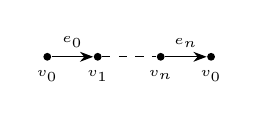
\begin{tikzpicture}[baseline=(v0.base), scale=0.8]
      \node[circle, fill, inner sep=1pt, label=below:{\tiny $v_0$}] (v0) at (0,0) {};
      \node[circle, fill, inner sep=1pt, label=below:{\tiny $v_1$}] (v1) at (0.8,0) {};
      \node[circle, fill, inner sep=1pt, label=below:{\tiny $v_n$}] (vn) at (1.8,0) {};
      \node[circle, fill, inner sep=1pt, label=below:{\tiny $v_0$}] (v0end) at (2.6,0) {};
      
      \draw[-{Stealth}] (v0) -- node[above] {\tiny $e_0$} (v1);
      \draw[dashed] (v1) -- (vn);
      \draw[-{Stealth}] (vn) -- node[above] {\tiny $e_n$} (v0end);
    \end{tikzpicture}
  }

  %%% Tikzcd
  % Set global style for all tikz-cd diagrams. All Math is to be in \displaystyle
\tikzcdset{
  every diagram/.append style={
    cells={font=\everymath\expandafter{\the\everymath\displaystyle}}
  }
}

\begin{document}
Simpson's non-abelian Hodge correspondence establishes a diffeomorphism between different moduli spaces of sheaves on a projective variety $X$ over the complex numbers.
Specifically, let $M_{n,Dol}^0(X)$ be the moduli space of semistable Higgs bundles of rank $n$ and degree $0$ on $X$ and let
\begin{equation}
M_{n,B}^0(X) \coloneqq \left\{ \Hom(\pi_1(X), GL_n) \right\} \modd GL_n
\end{equation} 
be the variety of $n$-dimensional representations of the fundamental group of $X$. Then Simpson's correspondence is a diffeomorphism
\begin{equation}
\varphi\colon M_{n,Dol}^0(X) \to M_{n,B}^0(X) \label{simpson correspondence}
\end{equation}
between these varieties, inducing therefore an isomorphism of their cohomology rings.
Since we are considering varieties over $\Cb$, the cohomology groups are endowed with mixed Hodge structures. But the morphism $\varphi$ is not algebraic and doesn't preserve the Hodge structures. Therefore, a natural question is to try and understand how $\varphi$ relates the Hodge structures.

In order to understand this, it is convenient to factor the pullback $\varphi^*$ into pieces that are easier to understand.
First of all, the Riemann-Hilbert correspondence establishes a diffeomorphism
\begin{equation}
M_{n,B}^0(X) \simeq M_{n, DR}^0(X)
\end{equation}
between the character variety $Rep(\pi_1(X), GL_n)$ and the De Rham moduli space, i.e. the moduli space parametrizing pairs $(\mc{E}, \nabla)$ where $\mc{E}$ is a vector bundle of rank $n$ on $X$ and
\begin{equation}
\nabla\colon \mc{E} \to \mc{E}\otimes\Omega_X
\end{equation}
is a flat connection on $\mc{E}$.

Simpson introduced the notion of $\lambda$-connection as a way to interpolate between connections and Higgs fields. For a fixed complex parameter $\lambda$, a $\lambda$-connection on a vector bundle $\mc{E}$ is a $\Cb$-linear morphism
\begin{equation}
\nabla_{\lambda}\colon \mc{E} \to \mc{E} \otimes \Omega_X,
\end{equation}
respecting the Leibniz rule up to the scalar $\lambda$, namely such that
\begin{equation}
\nabla_{\lambda}(f \cdot s) = f \cdot \nabla(s) + \lambda \, s \otimes \dd f.
\end{equation}
Notice that for $\lambda = 1$ we recover the notion of a connection, while for $\lambda = 0$ we get an $\O_X$-linear morphism $\mc{E} \to \mc{E}\otimes \Omega_X$, making $(\mc{E}, \nabla_0)$ into a Higgs bundle.

Let $M_{n, Hdg}^0(X)$ be the moduli space parametrizing triples $(\lambda, \mc{E}, \nabla)$, where $\lambda$ is a complex parameter, $\mc{E}$ is a rank $n$ and degree $0$ vector bundle on $X$ and $\nabla$ is a $\lambda$-connection on $X$. Th multiplicative group $\Gb_m$ acts on $M_{n, Hdg}^0(X)$ by scaling of $\nabla$. In particular, the projection $(\lambda, \mc{E}, \nabla) \mapsto \lambda$ defines a $\Gb_m$-equivariant morphism
\begin{equation}
f \colon M_{n, Hdg}^0(X) \to \Ab^1,
\end{equation}
where $\Gb_m$ acts on $\Ab^1$ with weight one. The fibers of $f$ over $0$ and $1$ are $M_{n, Dol}^0(X)$ and $M_{n, DR}^0(X)$ respectively, i.e. we have the following picture
\begin{equation}
\begin{tikzcd}
	{M_{n, Dol}^0(X)} & {M_{n,Hdg}^0(X)} & {M_{DR}} & {M_{n,B}^0(X)} \\
	{\{ 0 \}} & {\Ab^1} & {\{ 1 \}.}
	\arrow["i", hook, from=1-1, to=1-2]
	\arrow[from=1-1, to=2-1]
	\arrow["\lrcorner"{anchor=center, pos=0.125}, draw=none, from=1-1, to=2-2]
	\arrow["f", from=1-2, to=2-2]
	\arrow["j"', hook', from=1-3, to=1-2]
	\arrow["\psi", "\cong"', from=1-3, to=1-4]
	\arrow["\lrcorner"{anchor=center, pos=0.125, rotate=-90}, draw=none, from=1-3, to=2-2]
	\arrow[from=1-3, to=2-3]
	\arrow[from=2-1, to=2-2]
	\arrow[from=2-3, to=2-2]
\end{tikzcd} \label{moduli diagram}
\end{equation}
Using the fact that the morphism $f$ is $\Gb_m$-equivariant and that the fibers over all $\lambda \neq 0$ are isomorphic, one can show that $i$ and $j$ induce isomorphisms in cohomology. They are moreover algebraic maps, so they induce an isomorphism of mixed Hodge structures on between the cohomology of $M_{n,Dol}^0(X)$ and $M_{n, DR}(X)$. Finally, we need to understand how $\psi$ acts on the Hodge structures. In \cite[]{Shende-weights}, Shende approached this problem by replacing $X$ with a simplicial scheme $\Delta_X$ obtained by a trialeftngulation. The advantage of using this approach is that the simplicial scheme thus constructed admits an algebraic version of a universal local system, which can be used to compute the hodge weights.

Notice that the problem explained so far concerns only vector bundles of degree $0$. Indeed, in order for a vector bundle to admit a nontrivial flat connection, it needs to have degree $0$. On the other side, positive degree vector bundles can admit nontrivial Higgs fields, so we would like to have a version of \eqref{simpson correspondence} for positive degree Higgs bundles.
The purpose of this article is to study a version of \eqref{simpson correspondence} for vector bundles of nonzero degree in the case where $X$ is a genus $g$ curve and to apply Shende's technique to study the Hodge structure also in this case. Thanks to [Simpson], we know that in the degree $d$ case, the character variety in \eqref{simpson correspondence} should be replaced by
\begin{equation}
\left\{ (A_i, B_i) \in GL_n^{2g} \mymid \prod_{i=1}^{2g}[A_i, B_i]=e^{\frac{2 \pi i}{n} d} \right\} \modd \, GL_n. \label{stacky character variety}
\end{equation}
Our main contribution, is to interpret this space as character variety of a stacky curve, and use this interpretation to get an analogue of the picture described in \zcref{moduli diagram} and replicate Shende's argument.
Indeed, \eqref{stacky character variety} is a connected component of the variety of representations of the group
\begin{equation}
\left< a_i, b_i, c \mid i=1,\dots,g, \; \prod_{i=1}^g [a_i, b_i]=c, \; c^n=1 \right>.
\end{equation}
The key idea is that this group can be seen as the fundamental group of an orbifold curve with a singularity of order $n$, which algebraically corresponds to a stacky curve with a single stacky point with stabilizer $\mu_n$. If we let $\mc{X}$ be such a stacky curve, then we get the analogue of \eqref{moduli diagram}
\begin{equation}
\begin{tikzcd}
	{M_{n, Dol}^0(\mc{X})} & {M_{n,Hdg}^0(\mc{X})} & {M_{DR}} & {M_{n,B}^0(\mc{X})} \\
	{\{ 0 \}} & {\Ab^1} & {\{ 1 \}.}
	\arrow["i", hook, from=1-1, to=1-2]
	\arrow[from=1-1, to=2-1]
	\arrow["\lrcorner"{anchor=center, pos=0.125}, draw=none, from=1-1, to=2-2]
	\arrow["f", from=1-2, to=2-2]
	\arrow["j"', hook', from=1-3, to=1-2]
	\arrow["\psi", "\cong"', from=1-3, to=1-4]
	\arrow["\lrcorner"{anchor=center, pos=0.125, rotate=-90}, draw=none, from=1-3, to=2-2]
	\arrow[from=1-3, to=2-3]
	\arrow[from=2-1, to=2-2]
	\arrow[from=2-3, to=2-2]
\end{tikzcd} \label{moduli diagram stacky}
\end{equation}
The stacky curve $\mc{X}$ admits a line bundle $\O(\frac{1}{n})$of fractional degree, which we can use to twist degree $d$ vector bundles into degree $0$ vector bundles.
In particular, starting from a degree $d$ vector bundle $\mc{E}$ on $X$, we can pull it bach along $\pi\colon \mc{X} \to X$ and get a degree $d$ vector bundle on $\mc{X}$ with trivial type in the stacky point. After twisting, we get a vector bundle of degree $0$ on $\mc{X}$ which in the stacky point $p$ realizes the $\mu_n$-representation
\begin{equation}
\rho_n^{-d} \coloneqq 
\begin{pmatrix}
    \zeta_n^{-d} &  &  \\
     & \ddots &  \\
     &  & \zeta_n^{-d} \\
\end{pmatrix}.
\end{equation}

The described procedure lifts to an isomorphism of stacks
\begin{equation}
\mc{M}_n^d(X) \cong \mc{M}_{n, \text{triv}}^d(X) \cong \mc{M}_{n, \rho_n^{-d}}(\mc{X}),
\end{equation}
which extends to the various moduli stacks of vector bundles described above.
In particular, looking at the connected component of \eqref{moduli diagram stacky} determined by the invariants $(n, d, \rho_n^{-d})$, we recover a version of \eqref{simpson correspondence} for degree $d$ vector bundles on $X$.

Finally, we want to use \eqref{moduli diagram stacky} to compare the Hodge structures on $\mc{M}_{n, \rho_n^{-d}}(\mc{X})$ and on
\begin{equation}
\left\{ (A_i, B_i) \in GL_n^{2g} \mymid \prod_{i=1}^{2g}[A_i, B_i]=e^{\frac{2 \pi i}{n} d} \right\} \modd \, GL_n.
\end{equation}
In the case of \eqref{moduli diagram}, this was done by Shende in \cite[]{Shende-weights}, by replacing the complex manifold $X$ with a simplicial scheme $\Delta_X$ obtained from a triangulation of $X$. The key features of $\Delta_X$ are that its fundamental group coincides with the one of $X$, so it can be used to construct the stack of local systems on $X$, and that it has trivial Hodge Structure, giving the cohomology of moduli spaces on $\Delta_X$ an easier Hodge structure.
Explicitly, Shende uses an isomorphism
\begin{equation}
[\Hom(\pi_1(X), GL_n) / GL_n ] \cong \inHom_{SSch}(\Delta_X, BG)
\end{equation}
to study how \eqref{simpson correspondence} acts on the Hodge weights.

In the final part of the article, we replicate Shende's argument in the case we considered, by replacing the stacky curve $\mc{X}$ with a simplicial scheme $\Delta_{\mc{X}}$ realizing its fundamental group.


\printbibliography
\end{document}